\subsection{Rutherford's Model}

So a new model was required to explain the discrepencies away; in comes Rutherford.
He looked at the gold foil experiments done before him and ran with it, expanding upon them and developing a new theory on the substructure of the atom.
He proposed in 1911 that atoms were mostly just empty spacewith a highly concentrated segment of mass at the center of the atom -- he called this central mass the neucleus of the atom.
In Rutherford's atomic model, the electrons orbit around the positively charged neucleus.

\begin{figure}[H]
  % https://en.wikipedia.org/wiki/Rutherford_model#/media/File:Rutherford_atomic_planetary_model.svg
  \centering
  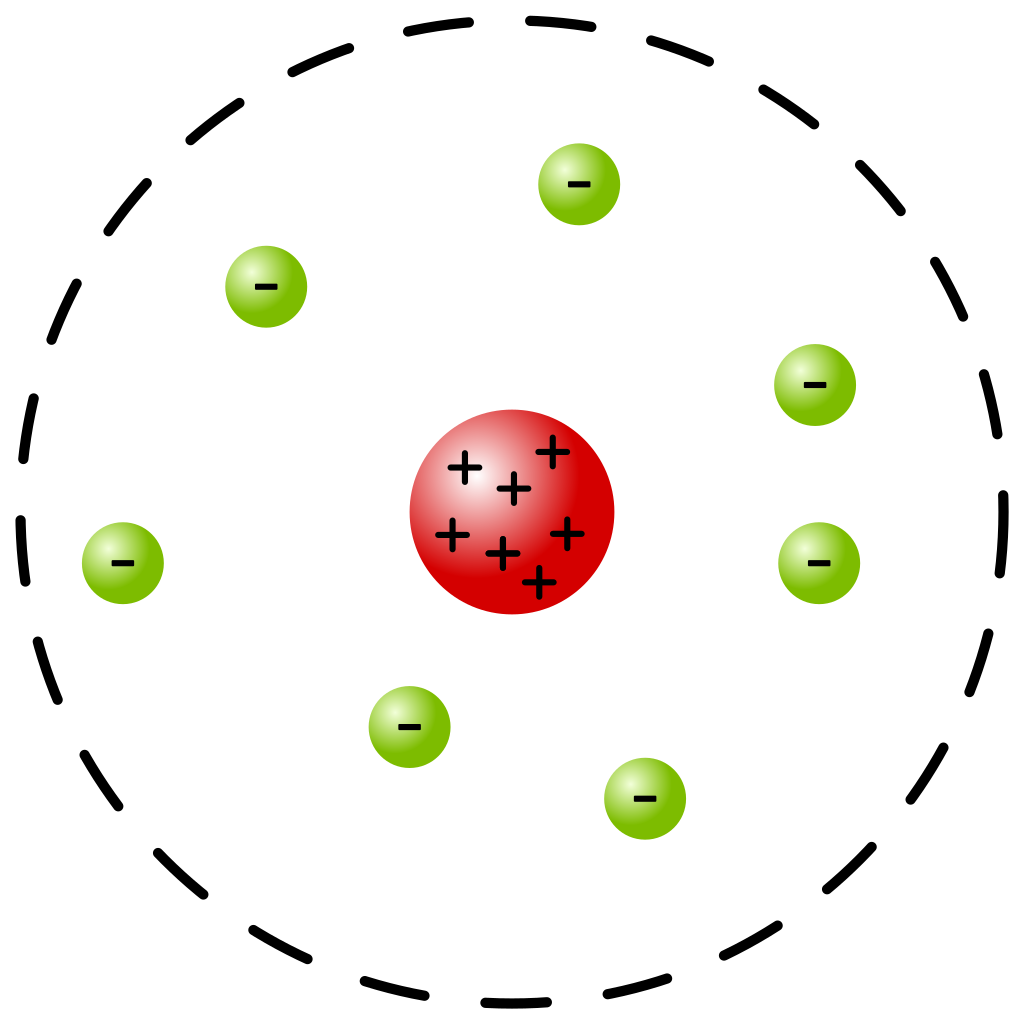
\includegraphics[width=100mm]{figures/rutherford.png}
  \caption{Rutherford's atomic model}
  \label{rutherford}
\end{figure}

Only, one little problem.
When things move in a circular orbit, they are accelerating and when a charged particle is moving in an orbit like that,  it should be constantly radiating energy leading to it eventually falling into the neucleus rendering this formulation of the atom unstable.
It should also be emitting a continous energy spectrum from the electrons, but hydrogen has discrete spectral lines.

